%%%%%%%%%%%%%%%%%%%%%%%%%%%%%%%%%%%%%%%%%%%%%%%%%%%%%%%%%%%%%%%%%%%%%%%%%%%%
%% Author template for Management Science (mnsc) for articles with e-companion (EC)
%% Mirko Janc, Ph.D., INFORMS, mirko.janc@informs.org
%% ver. 0.95, December 2010
%%%%%%%%%%%%%%%%%%%%%%%%%%%%%%%%%%%%%%%%%%%%%%%%%%%%%%%%%%%%%%%%%%%%%%%%%%%%
\documentclass[mnsc]{informs3b} % current default for manuscript submission
% \documentclass[man]{apa7}

%%\OneAndAHalfSpacedXI % current default line spacing
%%\OneAndAHalfSpacedXII 
%%\DoubleSpacedXII
%%\DoubleSpacedXI

% If hyperref is used, dvi-to-ps driver of choice must be declared as
%   an additional option to the \documentstyle. For example
%\documentclass[dvips,mnsc]{informs3}      % if dvips is used
%\documentclass[dvipsone,mnsc]{informs3}   % if dvipsone is used, etc.

% Private macros here (check that there is no clash with the style)

% \usepackage{lipsum}
% \usepackage[american]{babel}
% \usepackage{csquotes}

% \usepackage[style=apa,sortcites=true,sorting=nyt,backend=biber,natbib]{biblatex}
% \DeclareLanguageMapping{american}{american-apa}

% \addbibresource{zotero-refs.bib}
% \addbibresource{depression_attention.bib}

% \usepackage{comment}

% Natbib setup for author-year style

\usepackage{natbib}
 \bibpunct[, ]{(}{)}{,}{a}{}{,}%
 \def\bibfont{\small}%
 \def\bibsep{\smallskipamount}%
 \def\bibhang{24pt}%
 \def\newblock{\ }%
 \def\BIBand{and}%

 

% table related packages
% https://tex.stackexchange.com/questions/211898/putting-several-footnotes-below-the-table
\usepackage{booktabs, caption, makecell}
\renewcommand\theadfont{\bfseries}
\usepackage{threeparttable}
\usepackage{subcaption}
\usepackage{todonotes}
\usepackage{multirow}
\newenvironment{mytabular}[1][1]{%
  \setlength{\tabcolsep}{10pt}
  \renewcommand*{\arraystretch}{#1}%
  \tabular%
}{ \endtabular }
\newcommand{\blap}[1]{\smash[b]{\begin{mytabular}[1]{@{}l@{}}#1\end{mytabular}}}
\newcommand{\mr}[2]{\multirow[c]{#1}{*}{#2}}
\newcolumntype{M}[1]{>{\centering\arraybackslash}m{#1}}

\usepackage[resetlabels]{multibib}
\newcites{sec}{References}


%% Setup of theorem styles. Outcomment only one.
%% Preferred default is the first option.
\TheoremsNumberedThrough     % Preferred (Theorem 1, Lemma 1, Theorem 2)
%\TheoremsNumberedByChapter  % (Theorem 1.1, Lema 1.1, Theorem 1.2)
\ECRepeatTheorems

%% Setup of the equation numbering system. Outcomment only one.
%% Preferred default is the first option.
\EquationsNumberedThrough    % Default: (1), (2), ...
%\EquationsNumberedBySection % (1.1), (1.2), ...

% For new submissions, leave this number blank.
% For revisions, input the manuscript number assigned by the on-line
% system along with a suffix ".Rx" where x is the revision number.
% \MANUSCRIPTNO{MS-0001-1922.65}

\usepackage{amsmath}

\usepackage[bottom]{footmisc}
\usepackage{afterpage}

\usepackage{xcolor}

\usepackage[bookmarks, hidelinks]{hyperref}
\hypersetup{
	%	pdftitle={},
	%	pdfauthor={},
	%%	pdfsubject={},
	%%	pdfkeywords={},
	bookmarksnumbered=true,     
	bookmarksopen=true,
	bookmarksopenlevel=2,    
	colorlinks=true,
	linkcolor={red!50!black},
	citecolor={blue!50!black},
	urlcolor={blue!80!black},
	%	colorlinks=true,            
	%	pdfstartview=Fit,           
	%	pdfpagemode=UseOutlines,    % this is the option you were lookin for
	%	pdfpagelayout=TwoPageRight
}

\usepackage{bookmark}
\usepackage{etoolbox}
\usepackage{tocloft}
%%% Generate bookmarks for all figures and tables
\makeatletter
\pretocmd\endfigure{%
\addtocontents{lof}{\protect{%
    \bookmark[
    rellevel=1,
    keeplevel,
    dest=\@currentHref,
    ]{Figure \thefigure: \@currentlabelname}}}%
\bookmark[
rellevel=1,
keeplevel,
dest=\@currentHref,
]{Figure \thefigure: \@currentlabelname}%
}{}{\errmessage{Patching \noexpand\endfigure failed}}
\pretocmd\endtable{%
\addtocontents{lof}{\protect{%
    \bookmark[
    rellevel=1,
    keeplevel,
    dest=\@currentHref,
    ]{Table \thetable: \@currentlabelname}}}%
\bookmark[
rellevel=1,
keeplevel,
dest=\@currentHref,
]{Table \thetable: \@currentlabelname}%
}{}{\errmessage{Patching \noexpand\endtable failed}}
\makeatother

\usepackage{tabularx}
% for table formatting
% for horizontal table
\usepackage{lscape}

\usepackage{cases}
\usepackage{threeparttable}

\usepackage{comment}

% \usepackage{algorithm} 
\usepackage{algorithmic}
\usepackage[ruled,vlined]{algorithm2e}
\newcommand{\mytag}[1]{{\bf#1}}
\newcommand{\model}{DeepKnowledge}
\newcommand{\entity}{depression diagnosis-related entities}
\newcommand{\post}{user's generated contents}
% \usepackage[noend]{algpseudocode} 

% \usepackage{tikz}
% \usetikzlibrary{matrix}

% for annotated matrix
% https://www.overleaf.com/project/618957d82a1ed75a5fb0fd2c
\usepackage{blkarray}
\usepackage{bigstrut}

%turn numbering of theorem off
%\let\proof\relax
%\let\endproof\relax
%\usepackage{amsthm}
%conflict with the inform style

% define "struts", as suggested by Claudio Beccari in
%    a piece in TeX and TUG News, Vol. 2, 1993.
\newcommand\Tstrut{\rule{0pt}{2.6ex}}         % = `top' strut
\newcommand\Bstrut{\rule[-0.9ex]{0pt}{0pt}}   % = `bottom' strut
\newcommand{\red}[1]{\textcolor{red}{[#1]}}   % = `\red{}`


% the "APPENDICES" environment provided by the document class "informs3" doesn't work well with the package "hyperref", so we can try the alternative environment "appendices" provided by package
% "appendix" to add appendices, note that the two environment names are case sensitive
\usepackage[toc]{appendix}

%\pagestyle{plain}

\usepackage[nomessages]{fp}

% packages for writing the response section
\usepackage{enumitem}
%\usepackage{hanging}

\DeclareMathOperator{\dplus}{+\kern -0.4em+}

%newpackage
\usepackage{float}
\usepackage{graphicx}

% \DeclareUnicodeCharacter{2061}{}

%%%%%%%%%%%%%%%%
\begin{document}

\newcolumntype{L}[1]{>{\raggedright\arraybackslash}p{#1}}
\newcolumntype{C}[1]{>{\centering\arraybackslash}p{#1}}
\newcolumntype{R}[1]{>{\raggedleft\arraybackslash}p{#1}}


%\RUNTITLE{}


%\TITLE{Depression Detection Using Digital Traces on Social Media with Knowledge-driven Deep Learning}


%\ABSTRACT{
%}


% Fill in data. If unknown, outcomment the field
%\KEYWORDS{health analytics, depression, social media, digital trace, named entity recognition, knowledge-driven machine learning} 


\begin{center}
\textbf{\Large Depression Detection Using Digital Traces on Social Media with Knowledge-driven Deep Learning}    
\end{center}

\hspace{0.2cm}


\noindent \textbf{Abstract:} Depression is a common disease worldwide. It is difficult to diagnose and continues to be underdiagnosed. The past two decades have witnessed the rapid proliferation of social media. Researchers turn to social media data for depression detection because depression patients constantly share their symptoms, treatments, and self-reported causes of depression on social media. Social media has a distinct advantage in combating depression because it can provide personalized educational content, treatment options, and social support. However, most existing studies failed to incorporate established medical domain knowledge in depression detection and suffer from feature extraction difficulties that impede greater performance. We propose a new method to identify entities in social media posts directly related to depression diagnosis and use time-and-knowledge-aware LSTM to accurately detect social media users with depression or at risk of depressive disorders. Our work has significant implications for IS research in demonstrating how domain knowledge can be usefully incorporated into machine learning to create innovative and significant artifacts. Practically, the proposed method can supplement clinical depression screening and enable large-scale evaluations of a population's mental health status.



\noindent \textbf{Keywords:} health analytics, depression, social media, digital trace, named entity recognition, knowledge-driven machine learning

\hspace{1cm} 



% 
\section{Introduction}
\label{sec:intro}

The Fourth Industrial Revolution is characterized by technological advancements in high-speed Internet, artificial intelligence, big data analytics, and cloud computing~\citep{schwab_fourth_2017}. Along with its emergence and progress, numerous digital artifacts (e.g., sensors, tools, and information systems) capable of producing or collecting data are implemented by organizations worldwide to modernize their services, scale their business, or improve the efficiency of data exchange. Meanwhile, these digital artifacts record massive amounts of data describing the context and outcomes of users' actions and forming each user's unique digital traces~\red{not found Hedman, 2013}. As part of this trend, the digital traces of user-generated content on social media represent a massive and novel source of ecological data that describes human behaviors and psychological characteristics~\citep{foster_managing_2016, settanni_predicting_2018} which can be used for developing novel disease surveillance systems~\citep{wenli_zhang_comprehensive_2020}. 


In the 1st century, depression is one of the major contributors to the overall global disease burden\footnote{A concept developed by the Harvard school of public health, WHO, and the World Bank, which is used to calculate disability, premature death, and other factors.}. An estimated 3.8 percent of the world's population suffers from depression~\citep{who_who_2022}. In the United States (US), more than 21 million adults have had depression, representing 8.4\% of all US adults~\citep{nih_major_2022}, and approximately \$225 billion is spent on depression-related treatments and services every year~\citep{openminds_us_2019}. Meanwhile, depression is also the primary cause of lost productivity, with employers in the US losing more than \$23 billion each year as a result of its effects on absenteeism and presenteeism~\citep{nadeem_identifying_2016}\footnote{When employees are present for work but less productive due to their illness.}


Although considerable effort has been devoted to this research area, depression is still difficult to diagnose~\citep{andrade_epidemiology_2003}. First, there is no reliable laboratory test for diagnosing depression; the diagnoses are normally based on patients' self-reported experiences. Second, current electronic health record (EHR) systems lack tracking of behavioral data for effective depression detection. Third, people with depression have depressive and non-depressive episodes which further complicate accurate diagnosis. Meanwhile, depression continues to be underdiagnosed~\citep{prince_no_2007}. First, myths and misunderstandings cause individuals and primary care physicians to be unaware of depression symptoms. Second, the stigma associated with depression causes people to hide the issues and delay help-seeking. Third, people suffering from depressive disorders may be unable to access health care services due to a lack of transportation, financial resources, or insurance.

Improving approaches for detecting and surveilling depression is key to combating depression and has far-reaching health and societal implications. The rapid proliferation of social media and the associated social media users' digital traces open up new possibilities in depression detection. A diverse set of quantifiable signals relevant to depression, including self-reported diagnosis, causes, and symptoms, are observed on social media~\citep{coppersmith_measuring_2014,coppersmith_quantifying_2014, nadeem_identifying_2016}. Research suggests that health digital traces on social media provide a great means for capturing an individual's current states of mind, feelings, behaviors, and activities that often characterize depression~\citep{choudhury_predicting_2013,nadeem_identifying_2016}. Existing research shows that social media-based depression screening has the potential to achieve prediction results that are comparable to unaided clinician assessment and screening surveys~\citep{guntuku_detecting_2017}. Meanwhile, unlike traditional survey- or interview-based depression screening approaches, which take a snapshot of a patient's mental health conditions, social media-based techniques continuously collect digital traces that allow the tracking of an individual's mental health over time. Meanwhile, digital trace data enables non-reactive research, in which data is not generated through contact between researchers and subjects~\citep{salganik_bit_2019}, logging ``naturally" occurring evidence of social behavior or psychological traits. 

Using social media users' digital trace data, social media-based depression screening can facilitate novel approaches to fight depression and eventually relieve its social and economic burden. For social media users, such methods can provide early detection and raise awareness for those who are at risk of clinical depression. For social media platforms, depression screening techniques enable them to develop new services with personalized recommendations for users with depression (e.g., encourage the identified users to seek help and treatments; promote educational content and tools, treatment options, social support, etc.)\red{For public administration, xxx }

While promising, the current mainstream approaches for detecting depression on social media have major limitations. Most of these methods use feature engineering for depression detection. However, the adopted features, including LIWC, n-grams, and sentiment analysis~\citep{gautier_environmental_2017}\red{M's?}, do not specify clinical depression assessment, therefore deteriorating depression prediction performance. With the development of deep learning, an increasing number of researchers turn to end-to-end sequence models for depression detection using raw social media posts~\citep{lin_first_2020}\red{baseline table}. However, limitation persists due to depressive disorders largely displaying subtle and implicit changes in language and behavior, such as a switch in the types of topics~\citep{coppersmith_measuring_2014,coppersmith_quantifying_2014}. Such patterns are difficult to model unless massive labeled data is available for the training of deep learning models. A small group of researchers relies on social media users' online behaviors: e.g., the engagement of social media usage, the changes in egocentric networks~\red{Choudhury et al., 2013}, dictionary-based symptom and drug taggers~\citep{hussain_exploring_2020}. However, these predefined features do not align with the medical knowledge in depression diagnosis and do not significantly improve prediction performance. Moreover, the symptomatic episodes of depression come and go. Patients do not exhibit depressive symptoms consistently on social media. All the existing methods lack effective means of capturing the dynamic patterns that characterize depression.

To cope with the shortcomings of the previous approaches, guided by the medical knowledge in depression diagnosis, we devise a named entity recognition (NER) and knowledge-aware LSTM depression detection method using digital trace data on social media. Our work has important implications for information systems (IS) research. First, positioned in the computational design science research, we propose a knowledge-driven machine learning method that sheds light on other domain-knowledge-rich areas in IS, such as healthcare, finance, and legal research, in which domain knowledge can be meaningfully incorporated into machine learning to develop novel and impactful artifacts~\citep{abbasi_towards_2020}. The proposed method is our major contribution to the IS knowledge base~\citep{padmanabhan_machine_2022}. Second, the IT artifact of interest in this study is digital traces on social media, and we demonstrate that digital traces are valuable data sources for decision-making, particularly in healthcare analytics. Third, our work expands NLP research in IS, which is situated at the crossroads of design and data science and represents significant opportunities to develop effective artifacts that leverage unstructured digital trace data to address socio-technical concerns~\citep{yang_getting_2022,abbasi_big_2016}. Meanwhile, our work has significant practical implications for depression detection and surveillance. It provides an accurate prediction method that can provide complementary information to existing clinical depression screening procedures. From the perspective of public health and disaster management, our method can enable large-scale analyses of a population's mental health conditions beyond what has previously been possible with traditional methods.
% \section{Related Work} \label{sec:related}

\subsection{Healthcare predictive analytics in IS}\label{sec:related:one}

Healthcare predictive analytics examine patient data and make diagnostic or prognostic risk predictions~\citep{shmueli_predictive_2011}\red{TODO: not found,  Van Calster et al., 2019}. It is an important research area in IS~\citep{shmueli_predictive_2011} since the results of this research area have a wide range of important applications, such as identifying patients at risk~\red{TODO: Bardhan et al., 2015 not found; Lin et al., 2017 not found}, supporting clinical decision-making~\citep{ben-assuli_trajectories_2020}, and dealing with hospital administrative challenges~\citep{meyer_machine_2014}. Our study is within the domain of healthcare predictive analytics in IS: we seek to address the difficulties of accurate depression detection on social media platforms. 

Digital traces as a novel data source has significant potential and implications for addressing socio-technical concerns. Google is among the first organizations to conduct groundbreaking research using digital trace data (i.e., search queries from regions with a huge number of web search users) to detect influenza epidemics~\citep{ginsberg_detecting_2009}. Soon, leveraging digital trace data becomes an  emerging and vital research avenue in IS~\red{TODO: not found Agarwal et al., 2008; Hedman et al., 2013}. IS healthcare analytics researchers have used digital trace data to generate new data science artifacts to address healthcare challenges. For example,~\cite{wenli_zhang_comprehensive_2020} extract digital traces from social media, environmental sensors, and healthcare records to identify asthma risk factors. \red{TODO: not found Xie et al, 2022} retrieve patients' health digital traces to predict hospital readmissions. While academics have suggested that unique digital trace data combined with domain knowledge and appropriate analysis techniques can serve as the foundation for a ``21st-century science"~\red{TODO: not found Hedman et al., 2013; Watts, 2007}, they have also pointed out that IS researchers need new skills and tools to leverage digital trace data and exploit them effectively\red{TODO: not found Hedman et al., 2013}. Our work aligns with this research direction: we intend to design a new artifact that elevates medical knowledge to decipher digital trace data and identify patients at risk of clinic depression. 


\subsection{Depression detection using digital traces on social media}\label{sec:related:two}

Social media is normally defined as an Internet-based platform (e.g., Twitter). Social media has been extensively studied by IS and is seen as having tremendous potential in various IS regimes~\red{cite recent ISR misq social media based papers}. According to the uses and gratifications theory, the gratifications of using social media include expression of opinion, social interaction, information sharing or seeking, etc~\citep{whiting_why_2013}. Applying the network externalities and motivation theory,~\red{TODO: not found Lin \& Lu, 2011} show that enjoyment, peers, and usefulness explain why people continue to use social media. Especially, depressed patients are motivated to share their symptoms, treatments, and the self-believed causes of depression for offering or seeking support and fighting the stigma of mental illness, see~\ref{fig:Coopersmith}. Researchers who use social media for depression analyses mainly focus on two categories of studies: (1) the correlations between the use of social media sites and mental illness~\red{TODO: not found Aalbers et al., 2019; Keles et al., 2020}, and (2) using social media data for mental disorder detection~\citep{guntuku_detecting_2017}. Our work focuses on the latter aspect. 

\begin{figure}[h]
    \centering
    \noindent\includegraphics[width=0.6\textwidth]{imgs/Sample-Figure.pdf} 
    \caption{Todo: motivation: a synthetic example . search webmed, reddit, Twitter typical texts~\citep{coppersmith_adhd_2015,coppersmith_clpsych_2015}\red{is this a table or figure?}}
    \label{fig:Coopersmith}
\end{figure}

\begin{table}[h]
\centering
\caption{ Todo: motivation: a synthetic example. search webmed, reddit, Twitter typical texts }
\label{tb:Coopersmith}
\small
\begin{threeparttable}
    \begin{tabular}{L{80pt}C{100pt}C{100pt}C{100pt}}
    \toprule
    % \midrule
    Social media platforms    & Reddit & Twitter & WebMed \\ \midrule
    Social media users disclose depression-related symptoms, treatments, and causes.   & to fill  & to fill &  to fill \\
    \bottomrule
    \end{tabular}
\end{threeparttable}
\end{table}

As we mentioned, the majority of existing studies use sentiment analysis and lexicon-based features for depression detection~(see Table~\ref{tb:Michael}). For example, \red{TODO: not found Michael et al, 2020} conduct LIWC and sentimental analyses, followed by rule-based classification for finding people with emotional distress. Although practicable, there is a significant discrepancy between the features used in these studies and medical practitioners' criteria in depression detection. Most people experience low sentiments occasionally and certain individuals tend to favor specific words depending on their education level, the influence of peers, and social context. Sentiment analysis and lexicon-based features may provide insights to one's psychological states, but they do not specify clinical depression. 

\begin{table}[h]
\centering
\caption{Title here: table from the review paper; ICIS R2; Micael'}
\label{tb:Michael}
\small
\begin{threeparttable}
    \begin{tabular}{lL{100pt}L{150pt}L{75pt}L{15pt}} \toprule
    Study & Model & Novelty & Input &  TP\\ \midrule
    \red{paper one} & ProtoPNet & Prototype for image classification & An image &  No\\
    \red{paper two}& HPNet & Hierarchical prototype & An image &  No\\
    \red{paper three}& ProSeNet & Prototype for text classification & A piece of text & No \\
    
    Our Method& TempPNet & Capture temporal progression of the input & A sequence of walking tests & 
    % \checkmark
    Yes \\ \bottomrule
    \end{tabular}
\end{threeparttable}
\end{table}

A few prior studies consider entities in social media data that can characterize clinical depression. One of the first studies is by~\cite{coppersmith_measuring_2014,coppersmith_quantifying_2014}, in which the authors identify social media users' behavioral patterns, including social engagement and exercises. Similarly, \cite{choudhury_predicting_2013} examine social media users' behavior attributes, such as engagement in social media, the change in the egocentric social networks, emotional states, and depression-related topics. Although interesting and promising, the attributes used in these two studies still considerably differ from the medical definition of depression. As we know, depression has received concerted attention from many practitioners and researchers. There is established medical knowledge in depression detection and diagnosis, such as~\red{cite depression Scales cesd phq9 bdi} Our first research question (R1) is \textit{how to leverage medical domain knowledge for social media users' depression detection}. 

In 2020, \cite{hussain_exploring_2020} push this research area forward by proposing depression marker taggers to identify depression-related symptoms and drug-use experiences. This work is the closest to ours in motivation. However, this work and other existing studies use predetermined dictionaries and hand-crafted features, which limit their methods to find novel (e.g., model's unseen features), yet significant features for depression detection. Hence, we are motivated to automatically extract entities in social media posts directly related to clinic depression diagnoses, including depression symptoms, life events that may cause or exacerbate depression, and depression treatments~\citep{beck_depression_2014}. Our second research question (R2) is \textit{how to effectively extract depression diagnosis-related entities}.

Furthermore, depressed patients have depressive episodes, which are periods characterized by low mood and other depression symptoms that last for two weeks or more~\citep{beck_depression_2014}. Depressive episodes may occur from time to time. The existing methods do not capture the irregular time intervals of social media users' life patterns and behaviors. In the meantime, according to medical domain knowledge, different depressive symptoms indicate varying degrees of severity; different risk factors have different effects on the onset and exacerbation of depression. Such medical knowledge has not been taken into account by the previous approaches. Our third research question (R3) is \textit{how to incorporate knowledge (i.e., recency and relevancy to the onset of depression) associated with depression diagnosis-related entities for depression detection}.

\subsection{Knowledge-driven machine learning}\label{sec:related:three}

The last two decades have seen a dramatic rise in the applications of deep and complicated models with large-scale data, leading to the imprecise, even misleading, perception that the vast amount of valuable human knowledge acquired to date no longer matters. However, researchers in various fields have demonstrated that knowledge-driven machine learning, in which domain expertise or domain knowledge is explicitly and meaningfully incorporated in the design of machine learning models, can play an important role in many applications involving difficult learning tasks and limited training resources due to knowledge-driven machine learning models have clear advantages in streamlining model architectures, lowering training costs, and increasing model interpretability~\citep{hussain_exploring_2020}~\red{TODO: not found Rudin, 2022, Li, 2020}

In IS, knowledge-driven machine learning is starting to get more attention and has been used to design novel domain-dadapted machine learning artifacts. For example, \cite{yang_getting_2022} employ psycholinguistics theories to construct a framework that combines domain-adapted NLP artifacts with deep learning models to predict the individuals' personalities. 

In healthcare, the heterogeneity of patient cohorts, the complexity of medical knowledge, and the high needs for interpretability contribute to the complexity of healthcare-related learning tasks, where knowledge-driven machine learning can have enormous potentials~\red{TODO: not found Li, 2020}.

\red{our work xxx }.

\subsection{Knowledge-driven machine learning}\label{sec:related:four}

\subsubsection{Depression ontology (R1)}\label{sec:related:four:r1}

Ontology is the science of what is, including the types and structures of objects, properties, events, processes, and relationships~\citep{smith_ontology_2012}. Ontology is widely used in computer and information science to provide a standard vocabulary for researchers that need to share information. It provides machine-interpretable definitions of fundamental concepts of the domain and relations between the concepts~\red{not found: Musen, 2015}. 

In medical expert systems, ontology has been used to represent medical domain knowledge for disease diagnosis~\citep{zheng_ontology-based_2008}\red{not found: Arsene et al., 2011}. Additionally, uncertainty is widely acknowledged in medical expert systems. The Bayesian network and ontology have been utilized to describe clinical practice uncertainty for better decision-making~\citep{zheng_ontology-based_2008}. For depression detection, ontology-based approaches have been used to represent depression diagnosis terminologies~\citep{chang_depression_2013}\red{not found: Jung et al., 2017}. 

To address our first research question \textendash~leveraging medical domain knowledge for social media users' depression detection, we construct a depression ontology model that explicitly explains the terminologies used in depression diagnosis and treatments. We also incorporate the prevalence of these terminologies among depression patients into the ontology inference rule using the Bayesian network.

\subsubsection{Depression diagnosis-related entity identification (R2)}\label{sec:related:four:r2}

Named entity recognition (NER) is a well-suited approach to address the second research question \textendash~extracting depression diagnosis-related entities including depression symptoms, major life events, and depression treatments. NER is the task of identifying entities such as people, location, organization, drug, medical notions, etc~\citep{nadeau_survey_2007}.  NER is an essential step in most natural language processing tasks such as question answering, information retrieval, coreference resolution, and topic modeling, among others. Handcrafted rules, lexicons, orthographic features, and ontologies are used in early NER systems followed by feature engineering and machine learning techniques~\citep{nadeau_survey_2007}. Later, deep learning-based NER systems with minimal feature engineering grow in popularity. Such deep learning-based models are useful because they often do not require domain-specific resources (e.g., lexicons), making them more domain-independent~\citep{yadav_survey_2019}.

In this study, we adapt the state-of-the-art NER algorithm to identify the depression diagnosis-related entities in social media posts. According to the medical literature, the clinical diagnosis of depression is normally based on the chief complaint presented by depressed patients, including (1) symptoms, such as anxiety, fatigue, low mood, reduced self-esteem, change in appetite or sleep, suicide attempt, etc~\citep{apa_diagnostic_2013}; (2) major life event changes, such as divorce, body shape, violence, abuse, drug or alcohol use, and so on. We, therefore, use NER to discover depression symptoms and life events that may cause or exacerbate depression~\citep{beck_depression_2014}. Meanwhile, the mainstay of depression treatment is usually medication, therapy, or a combination of these two~\citep{mitchell_understanding_2008}. We also perform NER to locate antidepressants and depression therapies because they indicate the ongoing experience of depression. 

\subsubsection{Knowledge-aware LSTM for Depression Detection (R3)}\label{sec:related:four:r3}

\red{from Xie: If you want to use the ``knowledge-driven" concept, can we just call our method medical knowledge-driven LSTM? such medical knowledge includes time and medical ontology. I just feel it is weird to single out the ``time" concept, since we never emphasized it before. Time can be just another knowledge, because there are already many medical studies using time as additional knowledge for disease prediction Baytas et al. 2017, etc.}

Simulating the accumulation of recent/earlier and important/trivial (knowledge-driven) life events; and their impact on the development of depression. Such as depression diagnosis-related entities in this study, recurrent neural networks (RNN) are well-established approaches. An RNN is a deep learning method in which the hidden units are connected in a directed cycle, allowing the network to store past hidden states of information in the internal memory~\red{Bengio et al., 1994}. Long Short-Term Memory (LSTM) is a popular variant of RNN that has a gated structure to handle long-term dependencies~\red{Hochreiter \& Schmidhuber, 1997}. This study uses depression diagnosis-related entities as the inputs for depression detection. 

The recency and frequency of the depression diagnosis-related entities are important for depression detection. First, the occurrences of recent major life event changes are reported by the majority of patients with severe depression~\red{Heikkinen et al., 1994}. Second, LSTM assumes that there is a consistent consecutive property among the input elements, which does not hold in depression diagnosis-related entities for two reasons. (1) The frequency and the number of depression diagnosis-related entities that can be identified in social media data are variable and unstructured because of the irregularity of depressive episodes. (2) Missing information is common in the longitudinal social media data because social media users may not necessarily report their depression diagnosis-related symptoms, life events, and treatments. 

The relevancy of the depression diagnosis-related entities is also vital in detecting depression. According to medical domain knowledge~\red{APA, 2013}, different entities have varying relevance to depression diagnosis. For example, the entities we can identify on social media may be negative sentiments that do not necessarily indicate depression, because everyone can feel depressed, sad, or blue at some point in their lives. Entities like recurrent thoughts of death and excessive or inappropriate guilt, on the other hand, are strong indicators of depression. Depression diagnosis-related entities may also have varying effects on the onset and progression of depression. For example, traumatic events or major life changes can often trigger depression. Such knowledge (i.e., the relevancy of entities to depression) can be represented in the Bayesian network-based depression ontology. Nonetheless, the terminologies used in the depression ontology (i.e., medical terms) differ significantly from the entities identified on social media (i.e., informal language). We further apply the ontology alignment technique\red{Chu et al., 2020} to match the entities from social media and diagnosis terminologies in depression ontology.

Based on the assumption that more recent and relevant entities are more important in depression detection, we propose the time-and-knowledge-aware LSTM method to address our third research question \textendash characterizing the temporal and relevance information of depression diagnosis-related entities for depression detection.

\red{from Xie: i am still debating whether this is necessary in the lit review. But it depends on the length of the lit review. If it's too long, we can move it to the result section. before we show the attention results, just briefly explain what it is and what it can do}

\subsubsection{Summarization}\label{sec:related:four:summary}

todo

\section{Research Design}\label{sec:design}

In a given social media platform, we collect data from a user base $\mathcal{U}$. For a given period of time, we observe the digital traces of the focal user $u\in \mathcal{U}$ from $N$ social media posts, denoted by $p_1^u, p_2^u, \ldots, p_N^u$, ordered in time $\tau_1^u < \tau_2^u < \ldots < \tau_N^u$. Our objectives are two-folded: (1) We aim to detect all the \entity, denoted by $e_1^u, e_2^u, \ldots, e_M^u$, from a user's historical observations $\boldsymbol{H}^u = \left[\left(p_1^u, \tau_1^u\right), \left(p_2^u, \tau_2^u\right), \ldots, \left(p_N^u, \tau_N^u\right)\right]$. Here, the number of \entity, $M$, does not necessarily equal the number of social media posts $N$. One can extract zero, one or many \entity from a single social media post. (2) We aim to predict the probability of a user labeled as depression\footnote{we identify a depression user $u$ who has explicitly mentioned that they have been diagnosed with depression}. For simplicity, we describe our method for a given user $u$ and drop the superscript $u$ hereafter. The same analysis is applied to all the other users $\mathcal{U} \setminus u$. 

To achieve these two goals, we propose the DeepKnowledge Framework for Depression Detection (referred to as \model hereafter) from digital traces on social media. \model consists of three modules. 
The first module extracts the predefined entities that are informative of depression based on the medical knowledge (Section~\ref{sec:design:module1}). The second module establishes the medical knowledge foundation for our prediction and provides the source of depression knowledge for the third module (Section~\ref{sec:design:module2}). The third module leverages the knowledge from the first two modules and develops a knowledge-driven attention-based sequence model for depression prediction (Section~\ref{sec:design:module3}). 
The specific model components in these modules are shown in the first column in Table~\ref{tbl:design:knowledge}. The design rationale, the related medical knowledge, and the research gaps addressed for each model component are articulated in the second and third columns in Table~\ref{tbl:design:knowledge}. Figure~\ref{fig:design:model} shows the architecture of the proposed \model. 

\begin{table}[h]
    \caption{Notation} \label{tb:Notation}
    \small
    \centering
    \begin{threeparttable}
    \begin{tabular}{L{0.1\textwidth} L{0.85\textwidth}}
    \toprule
    Notation &  \multicolumn{1}{c}{Description} \\ \midrule
    $P_j$ & $j$-th social media posts of an individual \\
    $N_i$ & $i$-th diagnosis-related named entities of an individual\\
    $X_i$ & the BERT embedding of $i$-th named entitities of an individual \\
    $\tau_i$ & the time at which the post where $i$-th named entities belong is published \\
    \bottomrule
    \end{tabular} 
    \end{threeparttable}
    \end{table}

\begin{figure}[h]
    \centering
    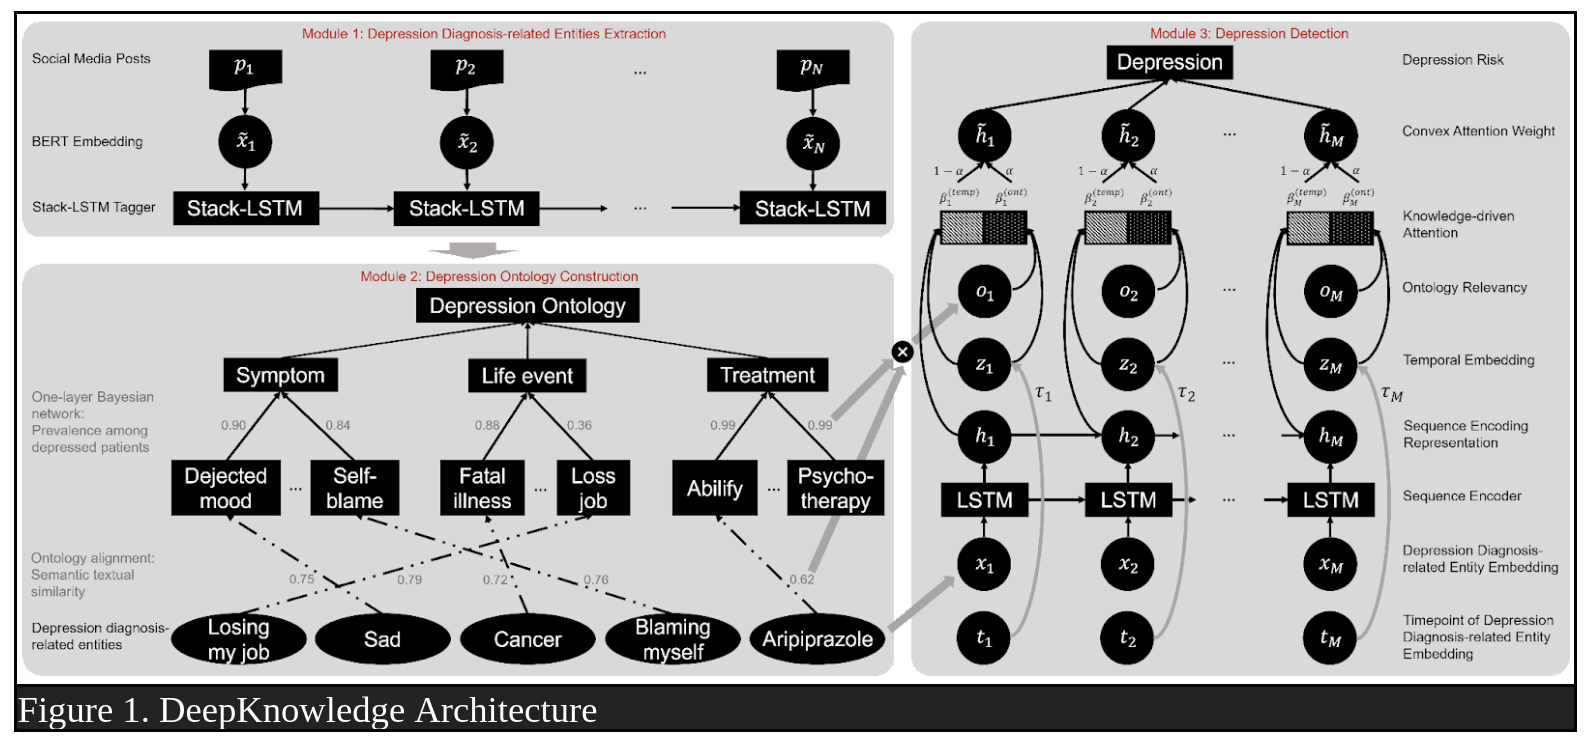
\includegraphics[width=1.0\textwidth]{imgs/method.png}
    \caption{The architecture of \model}
    \label{fig:design:model}
\end{figure}


\begin{algorithm}[!th]
%\small
% \footnotesize
\SetAlgoLined
    \textbf{Input:} Data $X=\{x_i\}_{i=1}^{N}$, labels $Y = \{y_i\}_{i=1}^{N}$ \\
    \textbf{Output:} $\Phi_{\Theta}$:targeted neural encoder for $X$, $U=\{u_c\}_{i=1}^{C}, V=\{v_c\}_{i=1}^{C}$: positive and negative anchors for each of $C$ classes\\
%\textbf{Output:} 
%%$Z_{A|B}$: conditional latent  representation for atoms,   %$Z_B$:latent representation for bonds, 
%$Z_M$:latent representation for atom $M$, 
%$\log P_\mathcal{M}(M)$: logarithmic  likelihood of molecule $M$. \\
%\KwResult{}
%\For{ \text{sampled mini-batch} $X=\{x_i\}_{i=1}^{N}$ }
\For{ each epoch }
{
    \mytag{Step 1:} Sampling mini-batch $X=\{x_i\}_{i=1}^{n}$ \\
    \mytag{Step 2:} Generating data representations $Z=\{z_i\}_{i=1}^{n} = \Phi(\{x_i\}_{i=1}^{n})$ \\
    \mytag{Step 3:} Computing  the supervised contrastive loss $\mathcal{L}_{\text{Supervised Contrastive} }  = \mathcal{L}_{\text{Contrastive Cross Entropy} }  + \lambda \mathcal{L}_{\text{Supervised Contrastive Regularizer}} $  by Eq.~\ref{eq:multi-cbce} or Eq.~\ref{eq:multi-csce} \\
    \mytag{Step 4:} Updating $\Theta, U, V$ by minimizing above loss. 
}
\quad \textbf{Return:} $\Phi_{\Theta}$, $U, V$\\
    \caption{ The learning framework of our \model \label{alg:scehr}}
\end{algorithm}

\begin{table}[h]
\centering
\caption{Design Guidelines for DeepKnowledge}~\label{tbl:design:knowledge}
\resizebox{\textwidth}{!}{
\begin{mytabular}[2]{L{2cm}L{2cm}m{8cm}m{5cm}}
    \toprule
    \multicolumn{2}{l}{Model Components} & Medical Knowledge & Research Gaps \\
    \midrule
    \multicolumn{2}{l}{\blap{Depression diagnosis-related \\ entities extraction}}
    & Depression diagnosis-related symptoms, life events, and treatments are critical indicators of depression and are essential for timely intervention~\citep{beck_depression_2014}.
    & Depression diagnosis-related symptoms, life events, and treatments are often overlooked in depression detection studies \\
    \multicolumn{2}{c}{\blap{Knowledge-driven depression\\ detection}}
    & Depression diagnosis-related symptoms, life events, and treatments are sequential data. Sequence encoders, such as LSTM, can model such time-series historical events~\citep{xie2022care}.
    & \multirow{7}{*}{\blap{Depression knowledge is \\ under-explored in machine \\ learning models for \\ depression detection.}} \\
    & Time & Time recency is essential knowledge to determine depression. More recent depression diagnosis-related symptoms, life events, and treatments have more salient influence than the older counterparts~\citep{heikkinen_recent_1994} & \\
    Depression knowledge & Ontology & Depression ontology information, including symptom, life event, and treatment, is indicative of depression risk~\citep{beck_depression_2014} & \\
    & Attention & Different depression diagnosis-related symptoms, life events, and treatments carry distinct influence on the depression risk. They can be weighted to provide an more accurate depression prediction~\citep{beck_depression_2014,xie_readmission_2021} & \\
    \bottomrule
\end{mytabular}
}
\end{table}



\subsection{Module 1: Depression Diagnosis-related Entities Extraction}\label{sec:design:module1}

Corresponding to the upper left block of Figure~\ref{fig:design:model}, we define \entity as personal encounters related to disease symptoms, major life events, and depression treatments. Figure~\ref{fig:design:extract} shows an example. To extract these entities from social media posts, we leverage a state-of-the-art transition-based NER model~\citep{lample_neural_2016}. This model has an architecture that chunks and labels a sequence of inputs using Stack-LSTM~\citep{dyer_transition-based_2015} which allows the NER model to work like a stack that maintains a “summary embedding” of its input. The text representation scheme of this model is BERT~\citep{devlin_bert_2018}. Let $\boldsymbol{P} = \left(p_1,p_2,\ldots, p_N\right)$ and $\boldsymbol{E} = \left(e_1,e_2,\ldots, e_M\right)$ be user's observed social media posts~\red{user generated contents sound better?} and extracted \entity respectively. The module learns a mapping: $\boldsymbol{P} \longrightarrow \boldsymbol{E}$. We also obtain the learnt language understanding representation for these \entity, $\boldsymbol{X} =\left(x_1,x_2,\ldots, x_M\right)$.  

\begin{figure}[h]
    \centering
    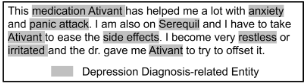
\includegraphics[width=0.4\textwidth]{imgs/example-ner.png}
    \caption{An example of \entity}
    \label{fig:design:extract}
\end{figure}

Unlike prior studies that use the entire social media post as the input, we leverage the detected \entity as our model input. These entities are more medically relevant and practically meaningful for explanation. Understanding what \entity are important in predicting depression is also critical for interventions. To name a few, if entities related to family emergencies are found to be salient predictors of the prediction, the social media platform can act on this information to offer online solutions for the emergencies and resources for support groups. If entities related to adverse drug events greatly contribute to the prediction, the platform can subsequently recommend guidelines from trusted health organizations (e.g., CDC, NIH, and WHO) on what actions to take to alleviate such adverse events. 


\subsection{Module 2: Depression Ontology Construction}\label{sec:design:module2}

The \entity extracted in module~\hyperref[sec:design:module1]{1} have uneven contributions to depression status~\red{uneven? equal contributions?}. Based on our depression ontology literature review, we construct a depression ontology as the medical knowledge base in our model. As shown in module~\hyperref[sec:design:module2]{2} of Figure~\ref{fig:design:model}, the medical terminologies used in the depression diagnosis can be divided into three subclasses~\citep{apa_diagnostic_2013,beck_depression_2014,almqvist_impact_2008}: Symptom, Life event, and Treatment. The Symptom class is a collection of depression symptoms. The Life event class is a collection of major life event changes that may cause or exacerbate depression. The Treatment class includes antidepressants and depression therapies.  The prevalence among depression patients is from the medical literature~\citep{beck_depression_2014}. The semantic textual similarity of each extracted \entity $e_i$ w.r.t the medical terminologies $mt_j$ corresponds to their dense representations inferred by the pre-trained language model $\phi$ (e.g., BERT~\citep{devlin_bert_2018}):

\begin{equation} \label{eq:cosine-similarity}
    \mathtt{sm}(e_i, mt_j) = \cos(\phi(e_i), \phi(mt_j))
\end{equation}

\subsection{Module 3: Time-Knowledge Fusion Depression Detection}\label{sec:design:module3}

Given a user's \entity sequence $\boldsymbol{X} = \left(e_1, e_2, \ldots, e_M\right)$ obtained from module~\hyperref[sec:design:module1]{1}, our goal is to predict the depression status of the focal user. The entity sequence encodes more relevant and practically more meaningful depression information than the original social media posts and creates a better user-level representation to identify depression. 

The right block of Figure~\ref{fig:design:model} shows the architecture of our proposed framework which can be break into three parts: 

The conventional LSTM model treats each depression diagnosis-related entity equally. Therefore, each entity would contribute equal information to the prediction. In reality, the importance of each entity based on the depression knowledge (i.e., relevancy to depression diagnosis and its time recency) is essential knowledge for this prediction. Based on this observation, DeepKnowledge embeds such depression knowledge into our sequence model. For each depression diagnosis-related entity $x_i$, we first learn an effective representation $h_i$ via an LSTM layer:

\begin{equation} \label{eq:lstm}
h_i = f^{(\mathtt{lstm})}\left(h_{i-1}, x_i\right)
\end{equation}


\section{Design Evaluation} \label{sec:eval}



Enter here

\section{Discussion and Future Research} \label{sec:discuss}

Enter here

\section{Conclusion} \label{sec:conclusion}

Enter here


% ---------------- main paper bib ------------------------

% \printbibliography


\bibliographystyle{informs2014} % outcomment this and next line in Case 1
\bibliography{depression_attention,zotero-refs} % if more than one, comma separated
\clearpage

\renewcommand{\theequation}{\arabic{equation}} 
\renewcommand{\thetable}{\arabic{table}}

\ECSwitch

% \ECHead{Supplementary Materials}
% \section{Chatbot}
\lstinputlisting[firstline=1, lastline=5]{index.js}

\section{Machine Learning}
\lstinputlisting[language=python, firstline=1, lastline=5]{model.py}


\end{document}
